%======================================================================
\subsection{BW-SIM-07 P2 --- Built, 1 Nov: parameters, named selections, local mesh sizes, study steps}\label{sec:sim07-p2-built}
%======================================================================

Phase P2 (plan answers W4 and W5) adds the \emph{Definitions} of a study and its \emph{steps}. The new code is two
headless modules, \file{bruceworx\_sim\_defs.py} (parameters, named selections, local sizes) and
\file{bruceworx\_sim\_steps.py} (steps), wired into the model layer, the Model Builder and the ribbon. One small C++
change: the Netgen mesh object of the Fem module has a new \code{MeshSizeFile} property.

\begin{figure}[!htbp]
\centering
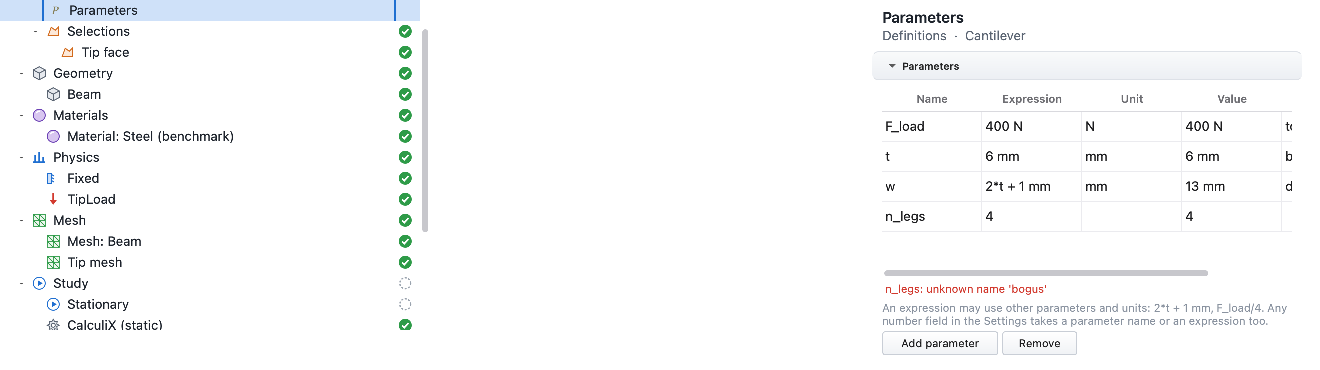
\includegraphics[width=\linewidth]{fig/simui_p2_params.png}
\caption{The cantilever with four parameters (off-screen render of the real window). The Parameters node shows the
table (name, expression, unit, value, description); \emph{n\_legs} was just edited into \code{bogus*2} and the error is
shown under the table; the value did not change. The Model Builder lists the named selection \emph{Tip face} and the local
size \emph{Tip mesh}; \emph{TipLoad} takes its faces from \emph{Tip face} and its force from \code{F\_load/n\_legs}.}
\label{fig:sim07-p2-params}
\end{figure}

\paragraph{What you can do now.}
\begin{itemize}[nosep]
  \item \textbf{Parameters.} Global Definitions $>$ Parameters is a table: name, expression, unit, evaluated value,
        description. An expression may use other parameters and units (\code{2*t + 1 mm}, \code{F\_load/4}); the unit
        column fixes the kind of the parameter (none, mm, N, MPa, deg, kg, s, \dots). Add and Remove are under the table
        (and in the right-click menu); an edit that fails (unknown name, a cycle, the wrong unit) shows the reason under the
        table and changes nothing; a parameter that a field uses cannot be removed (the message names the field).
  \item \textbf{Fields take expressions.} Every number field of the Settings form (loads, supports, mesh size, study
        step settings) accepts a parameter name or an expression: type \code{F\_load/4} in the
        Force field. The field then shows the expression (the value is in its tooltip) and the object holds the evaluated
        value; typing a plain value takes the field off the parameter again. Changing a parameter re-evaluates every field
        that uses it, in one undo step, and the fingerprints mark the right nodes out of date: a load parameter marks the
        solution and results, a mesh-size parameter the mesh as well; nothing is re-meshed or solved.
  \item \textbf{Named selections.} Global Definitions $>$ Selections: \emph{Selections} on the ribbon (or the right-click
        menu) makes one from the faces, edges or bodies selected in the 3D view. The node lists them and takes clicks in the
        3D view exactly as a load does. A load, a support or a local size has a \emph{Named selection} drop-down in its
        Settings: point several at the same one and an edit of the selection moves all of them. A linked object's own list is
        read only until you choose \emph{(own list)} again; deleting a selection leaves its users their faces.
  \item \textbf{Local mesh sizes.} Mesh $>$ \emph{Local size} (ribbon, right-click): a size in mm on the selected faces, edges
        or bodies, or on a named selection. Mesh feeds it to Netgen, so a hole or a fillet gets small elements without
        shrinking the whole mesh. A local size whose selection is shared with a load marks the mesh (and so everything after it)
        out of date when that selection changes.
  \item \textbf{Study steps.} The Study node of a study with more than one step has a child per step. \emph{Add step} (Study
        tab, right-click) appends one: \emph{Stationary} then \emph{Eigenfrequency} is a \emph{preload then modal} study (the
        modes about the loaded state, stress stiffening included, as a spinning rotor needs); \emph{Heat transfer} then
        \emph{Stationary} is the old thermal-stress study. A combination that is not supported is refused with the list of the
        supported ones. Each step has its own settings, and its own results: the preload's result is a node beside the modes;
        the temperatures are labelled Heat transfer and the stress Stationary.
  \item \textbf{Cancel and the mesh time limit (your answers of 1 Nov).} While a mesh or solve runs, the Compute button of the
        Mesh, Study, step and solver nodes reads \emph{Cancel}, and every running row of the Progress tab has a small stop button.
        Cancel kills the mesh worker (\code{bruceworx\_sim\_meshworker.cancel()}) and the CalculiX process. A worker mesh blocks
        the window's thread, so the worker's poll loop now calls a \code{PUMP} hook that the panes set to process events while
        a mesh runs (three lines in the worker module). The Mesh node shows \emph{Time limit: automatic (N min)} (the worker's
        rule on the node estimate) with an own limit field (\code{MeshTimeLimit}, seconds, 0 = automatic); an older study gets
        the property when its Mesh node is opened. The Gmsh choice is not shown yet: it is not in the model layer.
  \item \textbf{Old studies.} Steps are derived from the study type: an existing Static, Modal (prestressed or not), Buckling,
        Thermal or Thermal stress study opens unchanged, and shows its steps (a thermal-stress study is Heat transfer + Stationary
        and solves with two \code{*STEP} blocks now).
\end{itemize}

\paragraph{Decided while building.}
\begin{itemize}[nosep]
  \item \textbf{Storage: FreeCAD's expression engine, no spreadsheet.} The parameters are dynamic properties of one hidden
        \code{Parameters} object in the study's group (a Float for a plain number, the quantity property of its unit
        otherwise), so FreeCAD itself parses the expression, checks the units, refuses a cycle and re-evaluates dependent
        parameters on a recompute. A spreadsheet would add a cell grid and aliases that are not unit-checked, and an object that
        looks like a user document. The \emph{fields} are not bound with \code{setExpression}: the Netgen object would re-mesh
        on a recompute, and degC, rpm and whole-number fields would not work. A field stores its expression text in a hidden
        map on its object and \code{apply(study)} writes the evaluated value (through the holder's \code{evalExpression}: the
        same parser). \code{apply} runs after every parameter edit, before a pre-check, a mesh and a solve.
  \item \textbf{Parameter names that are units.} \code{t} (tonne), \code{h} (hour), \code{m}, \code{s} read as units in
        FreeCAD's parser, and \code{2*t+1 mm} is your own example. A parameter called \code{t} is stored as the property
        \code{t\_} and the expression is rewritten on the way in (\code{2*t}$\to$\code{2*t\_}); a unit right after a number
        stays a unit (\code{2 t} is two tonnes).
  \item \textbf{Named selections copy into the objects that use them.} The FEM writers read \code{References}; a hidden link
        \code{BW\_Selection} makes \code{sync(study)} copy the selection's references there (before the fingerprints, the
        pre-check and a solve). The writers, the highlight and the fingerprints stay untouched; the references are
        \code{PropertyLinkSubList}, so a named selection survives a recompute of the part exactly as a load does.
  \item \textbf{Local size through a Netgen size file.} The Netgen mesh object (\code{FemMeshShapeNetgenObject}, three lines
        of C++) now has a \code{MeshSizeFile} string, handed to Netgen's \code{SetMeshSizeFile}. Python samples points on the
        selected faces, edges or bodies and writes the \code{.msz} file (points \code{x y z h}); more than 60\,000 points
        is refused with the reason. Gmsh is not installed here, so the Gmsh route is not built. The mesh worker of the
        mesh-time work passes the property on.
  \item \textbf{Steps are a layer over the study types.} A step list maps to the existing study type (and back) instead of a new
        solver path: preload + modal is the prestressed modal study (\code{*STATIC}, then \code{*STEP, PERTURBATION} with
        \code{*FREQUENCY}); heat + stationary is the thermal-stress study, now written as \code{*HEAT TRANSFER, STEADY STATE}
        and \code{*STATIC} (the second step takes the temperatures of the first). Buckling and a transient heat run stay one
        step (the transient run is the Heat transfer step's own \emph{Time dependent} setting). Time dependent structural and
        steady CFD steps are not combinable yet.
\end{itemize}

\paragraph{Checks.}
\begin{itemize}[nosep]
  \item \textbf{Preload, then modal} (steel beam $500\times10\times10$\,mm, pinned ends, 10\,kN tension; built as an
        Eigenfrequency study, then the steps set to Stationary + Eigenfrequency): the first frequency is
        \textbf{146.60\,Hz} against the closed form of a tensioned beam $f_1=\tfrac{1}{2L}\sqrt{(T+\pi^2EI/L^2)/\rho A}$
        = \textbf{146.76\,Hz} (0.11\,\%); the same beam without the preload step gives 93.57\,Hz (closed form 93.81\,Hz).
        The input has two \code{*STEP} blocks, the second \code{*STEP, PERTURBATION}.
  \item \textbf{Heat transfer, then stationary} against the old thermal-stress study (steel bar 300\,mm held at both ends,
        +50\,K): mid-bar stress \textbf{$-127.356$\,MPa} with the two steps and with the old single block (identical to the
        printed digits), maximum von Mises 415.041 against 415.041\,MPa, the same maximum displacement, temperature and
        safety factor (all within $10^{-3}$ relative); the closed form $-E\alpha\Delta T=-126.0$\,MPa is 1.1\,\% away.
  \item \textbf{Local size} on the 10\,mm hole of a plate (global size 8\,mm, a hole size of 1\,mm): 5\,381 nodes become
        7\,517, and the nodes within 8\,mm of the hole's axis grow from 287 to 1\,725.
\end{itemize}

\paragraph{Tests.} \file{TestBruceWorxSimModel} (headless; 31 before, 45 now): parameters (a table with units and
derived values, expressions in a force and in the mesh size, a plain value taking the field off the parameter,
the stale marks, unknown name / wrong unit / cycle / reserved names with the document unchanged, undo, a removed
used parameter refused, save and reload), named selections (shared by two loads, an edit moving both, the own list read
only while linked, survives a change of the part, delete keeps the faces), local sizes (the refinement, the mesh mark
after a size or a shared selection changes, the file empty without one), steps (types of every study kind, the tree and
settings by step, adding and removing steps and converting back, one undo step, preload + modal and heat + stationary
against the references above). \file{TestBruceWorxSimWorkspace} (GUI, 28 before, 32 now): the parameter table and
the inline errors in the table and the field, the field with an expression following the table, named selection and local size
nodes (a click in the 3D view adding to the selection that a load uses), Add step, and the ribbon commands, the Cancel button and the Progress stop buttons, and the time-limit setting.
\file{TestBruceWorxSimCore}, \file{TestBruceWorxSimRotor}, \file{TestBruceWorxSimulation} and the validation fast set pass.

\paragraph{Open questions for you.}
\begin{enumerate}[nosep]
  \item \textbf{Rotor check.} The preload + modal reference is the tensioned beam, a closed form for the same mechanism (the
        stress stiffening). A spinning rotor's centrifugal stiffening needs the spin load in the first step; it is the same
        input, but I did not add a rotor reference (the rotor suite has the spin load and the modal study separately).
        Do you want one, and with which published case?
  \item \textbf{Several loads sets.} A load can use one named selection; two named selections on one load, or a selection of
        faces plus extra faces, need a union. Wanted?
  \item \textbf{Airflow studies} have no Parameters table yet (the holder is made for CalculiX studies); their number fields do not take
        expressions. Wanted in the next phase?
\end{enumerate}
